\pdfoutput=1

\documentclass[envcountsame]{llncs}
\usepackage[utf8]{inputenc}
\usepackage{amsmath}

\usepackage{multirow}
\usepackage{amssymb}
\usepackage{stmaryrd}
\usepackage{booktabs}
\usepackage{xspace}
\usepackage{placeins}
\usepackage{enumerate}
\usepackage{verbatim}
\usepackage{enumerate}
\usepackage{mathtools}
\usepackage{url}
\usepackage{thm-restate}
\usepackage{color}
\usepackage{subfigure}
\usepackage{wrapfig}


\usepackage[bookmarks=false]{hyperref}

\newcommand\sem[1]{\llbracket #1 \rrbracket}
\newcommand\inter[1]{\llbracket #1 \rrbracket}
\newcommand\trans[2]{\ensuremath{#1\mid #2}}
\newcommand\delay{\Delta}
\newcommand\tra{\mathcal{T}}
\newcommand\eof{\hfill}

\usepackage{graphicx}

\usepackage{xcolor,pgf,tikz}
\usetikzlibrary{arrows,automata,decorations.pathmorphing,snakes}



\title{
Multi-Sequential Word Relations}


\author{
Ismaël Jecker\and
Emmanuel Filiot
}
\institute{
Université Libre de Bruxelles}



\pagestyle{plain}

\begin{document}
\maketitle

\begin{abstract}
    Rational relations are binary relations of finite words that are
    realised by non-deterministic finite state transducers (NFT). 
    A particular kind of rational relations is the sequential
    functions. Sequential functions are the functions that can be
    realised by input-deterministic transducers. Some rational
    functions are not sequential. However, based on a property on
    transducers called the twinning property, it is decidable in
    \textsc{PTime} whether a rational function given by an NFT is
    sequential. In this paper, we investigate the
    generalisation of this result to multi-sequential relations,
    i.e. relations that are equal to a finite union of sequential
    functions. We show that given an NFT, it is decidable in
    \textsc{PTime} whether the relation it defines is
    multi-sequential, based on a property called the weak twinning
    property. If the weak twinning property is satisfied, we give a procedure that effectively
    constructs a finite set of input-deterministic transducers whose
    union defines the relation. This procedure generalises to
    arbitrary NFT the determinisation procedure of 
    functional NFT.
\end{abstract}



Finite transducers extend finite automata with 
output words on transitions. Any successful computation (called run) of a
transducer defines an output word obtained by concatenating, from
left to right, the words occurring along the transitions of that
computation. Since transitions are non-deterministic in general, there
might be several successful runs on the same input word , and hence 
several output words associated with . Therefore, finite
transducers can define binary relations of finite words, the so-called
class of rational relations \cite{Elgot:Mezei:ibmjrd:1965,berstel2009}.
Unlike finite automata, the equivalence problem, i.e. whether two transducers define the same
relation, is undecidable \cite{DBLP:journals/jacm/Griffiths68}. This has
motivated the study of different subclasses of rational relations, and
their associated definability problems: given a finite transducer ,
does the relation  it defines belong to a given class
 of relations? We survey the most
important known subclasses of rational relations. 


\paragraph{Rational Functions} An important subclass of rational relations is the class of
\emph{rational functions}.  It enjoys decidable
equivalence and moreover, it is decidable whether a transducer
is functional, i.e. defines a function. This latter result was first shown by 
Sch\"utzenberger with polynomial space complexity \cite{Schutz75} and the complexity has been refined to
polynomial time in \cite{GurIba83,BealCPS03}.


A subclass of rational functions which enjoys good algorithmic
properties with respect to evaluation is the class of \emph{sequential
  functions}. Sequential functions are those functions defined by 
finite transducers whose underlying input automaton is deterministic
(called sequential transducers). Some rational functions are not
sequential. E.g., over the alphabet , the 
function  mapping any word of the form  to , where
 and , is rational but not sequential,
because finite transducers process input words from left-to-right, and
therefore any transducer implementing that function should
 guess non-deterministically the last symbol of . 
Given a functional transducer, it is decidable whether it defines a
sequential function \cite{DBLP:journals/tcs/Choffrut77}, based on a
structural property of finite transducers called the \emph{twinning
  property}. This property can be decided in \textsc{PTime}
\cite{BealCPS03} and therefore, deciding whether a functional
transducer defines a sequential function is in
\textsc{PTime}. If the twinning property holds, one can
``determinise'' the original transducer into an equivalent sequential
transducer. 



It turns out that many examples of rational functions from the
literature which are not sequential are \emph{almost} sequential, in
the sense that they are equal to a finite union of sequential
functions. Such functions are called \emph{multi-sequential}. 
For instance, the function  is multi-sequential, as
, where  is
the partial sequential function mapping all words of the form  to
 (and similarly for ). Some rational functions are not
multi-sequential,  such as functions that are iterations of non-sequential functions. E.g., the function 
mapping  to  for some separator , is not multi-sequential. 
Multi-sequential functions have been
considered by Choffrut and
Sch\"utzenberger in \cite{DBLP:conf/stacs/ChoffrutS86}, where it is shown
that multi-sequentiality for functional transducers is a decidable
problem. 

\paragraph{Contribution} In this paper, we investigate multi-sequential relations,
i.e. relations that are equal to a finite union of sequential functions. Our
main result shows that, given a finite transducer, it is decidable in
\textsc{PTime} whether the relation it defines is
multi-sequential. Our procedure is based on a simple characterisation
of multi-sequential relations by means of a structural property,
called the weak twinning property (WTP), on finite transducers. We
show that a finite transducer defines a multi-sequential relation iff
it satisfies the WTP. We define a ``determinisation'' procedure of
finite transducers satisfying the WTP, that decomposes them into finite
unions of sequential transducers. Finally, we also investigate the
computational properties of multi-sequential relations and show, that,
for a natural computational model for word relations, 
multi-sequential relations correspond to the relations that
can be evaluated with constant memory.


\paragraph{Related Works} As already mentioned, multi-sequential
functions were considered in \cite{DBLP:conf/stacs/ChoffrutS86}. Our
weak twinning property is close to the characterisation of
multi-sequential functions of \cite{DBLP:conf/stacs/ChoffrutS86}, which is based on analysing 
families of \emph{branching paths} in transducers. Thanks to the
notion of \emph{delay} between output words, our property is simpler
and can be decided in \textsc{PTime}, for arbitrary (not
necessarily functional) transducers. Compared to
\cite{DBLP:conf/stacs/ChoffrutS86}, our decomposition procedure is
more constructive. It extends the known determinisation procedure of
functional transducers, to multi-sequential relations, and applies
directly on arbitrary finite state transducers (in
\cite{DBLP:conf/stacs/ChoffrutS86}, the functional transducers are assumed to be
unambiguous, but removing ambiguity is worst-case exponential). 



Finite-valued rational relations are rational relations such that any
input word has at most  images by the relation, for a fixed
constant . Finite-valuedness (existence of such a ) is decidable in \textsc{PTime} for
rational relations, and any -valued rational relation is equal to a
union of  rational functions \cite{journals/mst/SakarovitchS10,SICOMP::Weber1993,DBLP:journals/acta/Weber89}. 
Equivalence of finite-valued rational relations is decidable
\cite{GurIba83}. Clearly, any multi-sequential relation is
finite-valued. However, for the multi-sequentiality problem, it would
not have been simpler to assume that the input relation is given as a
finite union of rational functions, because obtaining such as
decomposition is costly, and moreover, our property is simpler than the structural properties 
of \cite{journals/mst/SakarovitchS10,DBLP:journals/acta/Weber89} that 
characterise finite-valuedness.




Finally, finitely-sequential relations have been considered in
\cite{DBLP:journals/ijfcs/AllauzenM03}. They correspond to relations
that can be realised by an input-deterministic transducer whose
accepting states can, at the end of the run, output additional words
from a finite set. Such relations are much weaker than
multi-sequential relations. 


The known and new results of this paper are summarised in
Table~\ref{table:summary}. 


\begin{table}[t]
    \centering
    \begin{tabular}{c|c|c|c|c}
\toprule
sequentiality & multi-sequentiality  & functionality & multi-sequentiality & finite-valuedness \\
 & (for functions) &  & 
\\\midrule
\textsc{PSpace} \cite{DBLP:journals/tcs/Choffrut77} & \textsc{Decidable} \cite{DBLP:conf/stacs/ChoffrutS86} & \textsc{PSpace}
                                                  \cite{Schutz75} &
                                                           \textsc{PTime}
                                                           (\textbf{this
      paper}) & \textsc{PTime} \cite{journals/mst/SakarovitchS10,DBLP:journals/acta/Weber89} \\
\textsc{PTime} \cite{BealCPS03} & \textsc{PTime} (\textbf{this paper}) & \textsc{PTime}
                                                  \cite{GurIba83,BealCPS03}&
                                                           & \\
\bottomrule
\end{tabular}
\caption{\label{table:summary}Definability problems for rational relations given by finite transducers}\label{tab}
\vspace{-9mm}
\end{table}



\vspace{-4mm}
\section{Rational Word Relations}
\vspace{-2mm}

We denote by  the set of natural numbers
, and by  the set of subsets of
a set , and by  the set of finite subsets of .  



\vspace{2mm}
\noindent \textbf{Words and delays} Let  be a (finite)
alphabet of symbols. The elements of the free monoid  are
called words over . The length of a word  is written .
The free monoid  is partially ordered by the prefix relation
. We denote by  the set of
symbols  for all . Any word  can be reduced into an irreducible word  by the equations
 for all
. Let  be the set of irreducible words over
. The set  equipped with concatenation  is a group, called the free group over . We denote by  the inverse
of . E.g. . The \emph{delay} between two words  and  is the element
. E.g., . 


\vspace{2mm}
\noindent \textbf{Finite automata} A (finite) automaton
over a monoid  is a tuple  where  is the finite set
of states,  is the set of initial states, 
is the set of final states, and  is the
finite set of edges, or transitions, labelled by elements of the monoid .

For all transitions ,  is called the source of ,  its target and  its label.
A run of an automaton is a sequence of transitions  such that for every , the target of  is equal
to the source of . We write  (or just  when it is clear from the context) to mean
that there is a run  such that  is the source of
,  the target of , and  is the product of the labels
of the . A run is called accepting if its source is an initial state and its target is a final state.
An automaton is called trim if each of its states occurs in at least
one accepting run. It is well-known that any automaton can be trimmed
in polynomial time. The language recognised by an automaton over a monoid  is the set of elements of  labelling its accepting runs.
A -automaton is an automaton over the free monoid  such that each edge is labelled by a single element  of .
A -automaton is called deterministic if it has a single initial state,
and for all  and , there exists at most one
transition labelled  of source .

Given two automata  and  over a monoid , their disjoint
union  is defined as the disjoint union of their set of states, initial and final states,
and transitions. It recognises the union of the their respective
languages. 

\vspace{2mm}
\noindent \textbf{Finite transducers} Let  and  two
alphabets. A (finite)
transducer  from  to  is a tuple
 such that  is a
finite automaton over the monoid , called the underlying automaton of ,
such that , 
and  is the final output
function. In this paper, the input and output alphabets are always denoted by
 and . Hence, we just
use the terminology transducer instead of transducer from 
to . 



A run (resp. accepting run) of  is a run (resp. accepting run)
of its underlying automaton. We write  instead
of . The relation recognised by  is the
set  of pairs  such that  for  and . A transducer  is functional if  is a function. It is called trim if its underlying automaton is trim.
The input automaton of a transducer is the -automaton obtained by projecting the labels of its underlying automaton on their first component.
Given a transducer , we denote by  the
maximal integer , , such that  labels a
transition of  or  for some . 

A rational transducer is defined as a transducer, except that its
transitions are labeled in . Rational
transducers are strictly more expressive than transducers and define
the class of rational relations. E.g., by using loops 
, a word can have infinitely many images
by a rational relation. If there is no such loop, it is
easily shown that rational transducers are equivalent to transducers\footnote{Transducers are sometimes called real-time in the
  literature, and rational transducers just transducers. To avoid
  unecessary technical difficulties, we establish our main result for 
  (real-time) transducers, but, as shown in Remark \ref{rm:realtime},
  it still holds for rational transducers.}. 




\vspace{-3mm}
\section{Multi-Sequential Relations}
\vspace{-2mm}

In this section, we define multi-sequential relations, and give a
decidable property on transducers that characterise them.

\vspace{-4mm}
\subsection{From sequential functions to multi-sequential relations}
\vspace{-2mm}

A transducer  is
\emph{sequential} if its input automaton is deterministic. A function  is
\emph{sequential} if it can be realised by a sequential
transducer\footnote{These functions are sometimes called subsequential
in the literature. We follow the terminology of
\cite{DBLP:books/daglib/0023547}.}, i.e.  for
some sequential transducer . 

\begin{figure}[t]
\centering
\subfigure[\label{ex1}]{
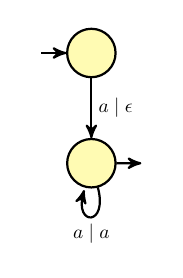
\begin{tikzpicture}[->,>=stealth',auto,node distance=2cm,thick,scale=0.7,every node/.style={scale=0.7}]
  \tikzstyle{every state}=[fill=yellow!30,text=black]
\tikzstyle{initial}=[initial by arrow, initial where=left, initial text=]
  \tikzstyle{accepting}=[accepting by arrow, accepting where=right, accepting text=]

  \node[initial,state] (A)  {};
  \node[accepting,state] (B) [below of=A] {};
  \path (A) edge node {\trans{a}{\epsilon}} (B);
  \path (B) edge [loop below] node {\trans{a}{a}} (B);
\end{tikzpicture}
}\subfigure[\label{ex2}]{
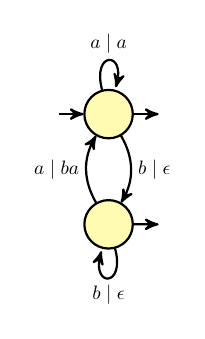
\begin{tikzpicture}[->,>=stealth',auto,node distance=2cm,thick,scale=0.7,every node/.style={scale=0.7}]
  \tikzstyle{every state}=[fill=yellow!30,text=black]
\tikzstyle{initial}=[initial by arrow, initial where=left, initial text=]
  \tikzstyle{accepting}=[accepting by arrow, accepting where=right, accepting text=]

  \node[initial,accepting,state] (A)  {};
  \node[accepting,state] (B) [below of=A] {};
  \path (A) edge [bend left] node {\trans{b}{\epsilon}} (B);
  \path (B) edge [bend left] node {\trans{a}{ba}} (A);
  \path (A) edge [loop above] node {\trans{a}{a}} (A);
  \path (B) edge [loop below] node {\trans{b}{\epsilon}} (B);
\end{tikzpicture}
}\subfigure[\label{ex3}]{
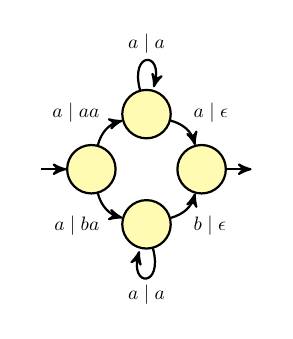
\begin{tikzpicture}[->,>=stealth',auto,node distance=2cm,thick,scale=0.7,every node/.style={scale=0.7}]
  \tikzstyle{every state}=[fill=yellow!30,text=black]
\tikzstyle{initial}=[initial by arrow, initial where=left, initial text=]
  \tikzstyle{accepting}=[accepting by arrow, accepting where=right, accepting text=]

  \node[initial,state] (A) at (0,0) {};
  \node[state] (B) at (1,1) {};
  \node[state] (C) at (1,-1) {};
  \node[state,accepting] (D) at (2,0) {};

  \path (A) edge [bend left] node {\trans{a}{aa}} (B);
  \path (B) edge [bend left] node {\trans{a}{\epsilon}} (D);
  \path (A) edge [below left,bend right] node {\trans{a}{ba}} (C);
  \path (C) edge [below right,bend right] node {\trans{b}{\epsilon}} (D);
  \path (B) edge [loop above] node {\trans{a}{a}} (B);
  \path (C) edge [loop below] node {\trans{a}{a}} (C);
\end{tikzpicture}
}\subfigure[\label{ex4}]{
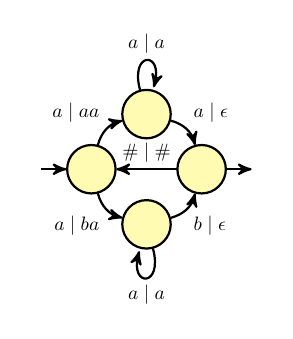
\begin{tikzpicture}[->,>=stealth',auto,node distance=2cm,thick,scale=0.7,every node/.style={scale=0.7}]
  \tikzstyle{every state}=[fill=yellow!30,text=black]
\tikzstyle{initial}=[initial by arrow, initial where=left, initial text=]
  \tikzstyle{accepting}=[accepting by arrow, accepting where=right, accepting text=]

  \node[initial,state] (A) at (0,0) {};
  \node[state] (B) at (1,1) {};
  \node[state] (C) at (1,-1) {};
  \node[state,accepting] (D) at (2,0) {};

  \path (A) edge [bend left] node {\trans{a}{aa}} (B);
  \path (B) edge [bend left] node {\trans{a}{\epsilon}} (D);
  \path (A) edge [below left,bend right] node {\trans{a}{ba}} (C);
  \path (C) edge [below right,bend right] node {\trans{b}{\epsilon}} (D);
  \path (B) edge [loop above] node {\trans{a}{a}} (B);
  \path (C) edge [loop below] node {\trans{a}{a}} (C);
  \path (D) edge [above] node {\trans{\#}{\#}} (A);
\end{tikzpicture}
}
\vspace{-4mm}
\caption{Finite transducers}
\label{fig:transducers} 
\vspace{-6mm}
\end{figure}


Let . Fig. \ref{fig:transducers} depicts transducers 
that implement sequential and non-sequential functions. All states
which is the target of a source-less arrow are initial, and those
which are the source of an arrow without target, or whose target is a
word, are accepting.  The function  that maps any word of the
form , , to , is sequential. It is realised by the
transducer of Fig.~\ref{ex1}. The function  replaces each
block of consecutive  by a single , but the last
one. E.g. . It is sequential and defined by
the sequential transducer of Fig.~\ref{ex2}. The function 
maps any word of the form  to , for
. It is not sequential, because the transducer
has to guess the last symbol . It can be defined by the
transducer of Fig.~\ref{ex3}. 



Sequential functions have been characterised by a structural property
of the transducers defining them, called the \emph{twinning
  property}.  Precisely, a trim transducers with initial state 
is twinned iff for all states , all words  and
, if  and , then . E.g., by taking , ,  and , it is easy to see that 
the transducer of Fig.\ref{ex3} is not twinned.


\begin{theorem}[\cite{DBLP:journals/tcs/Choffrut77,BealCPS03}]
Let  be a trim transducer.
\vspace{-2mm}
\begin{enumerate}
    \item  is twinned iff  is sequential. 
    \item It is decidable in \textsc{PTime} whether a trim transducer
      is twinned. 
\end{enumerate}
\end{theorem}


The following result is a folklore result that we show in Appendix for the
sake of completeness. It states that the difference
(the delay) between the outputs of 
two input words is linearly bounded by the difference of their
input words. 
  
\vspace{-1mm}
\begin{proposition}\label{bounded_variation}
Let  be a sequential transducer. For all pairs , .
\end{proposition}

\vspace{-4mm}
\paragraph{Multi-sequential relations} The function  is not
sequential, but it is multi-sequential, in the sense that it is the
union of two sequential functions  such that  is the
restriction of  to words in  and  its restriction
to words in . Precisely:

\begin{definition}[Multi-sequential relations]
    A relation  is
    multi-sequential if there exist  sequential functions
     such that . 
\end{definition}

The \emph{multi-sequentiality problem} asks, given a transducer ,
whether  is multi-sequential. It should be clear that
the answer to this problem is not always positive. Indeed, even some
rational functions are not multi-sequential. It is the case
for instance for the function  that maps any word of the
form  to , where  and  is a
fresh symbol. This function is rational, as it can be defined by the
transducer of Fig.~\ref{ex4}. In this paper, we investigate the intrinsic reasons
making a rational relation like  multi-sequential and a
rational relation like  not. In particular, we define a
weaker variant of the twinning property that characterises the
multi-sequential relations by structural properties of the transducers
which define them. 

\vspace{-5mm} 
\subsection{Weak Twinning Property}
\vspace{-1mm} 

\begin{definition}\label{def:wtp}
    Let  be trim transducer and  be two
    states of . We say that  is weakly twinned to
     if for all words
     and all words , if , or graphically
\begin{center}
\vspace{-1mm}
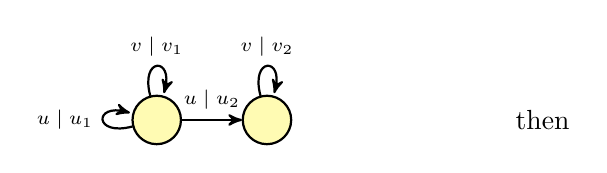
\begin{tikzpicture}[->,>=stealth',auto,node distance=2cm,thick,scale=0.7,every node/.style={scale=0.7}]
  \tikzstyle{every state}=[fill=yellow!30,text=black]
\tikzstyle{initial}=[initial by arrow, initial where=left, initial text=]
  \tikzstyle{accepting}=[accepting by arrow, accepting where=right, accepting text=]

  \node[state] (A)  {};
  \node[state] (B) [right of=A] {};
  \tikzstyle{every node}=[font=\normalsize]
  \node[] (C) [right of=B,xshift=1.5cm] {then };
  \tikzstyle{every node}=[font=\scriptsize]
  \path (A) edge [loop above] node {\trans{v}{v_1}} (A);
  \path (A) edge [loop left] node {\trans{u}{u_1}} (A);
  \path (A) edge node {\trans{u}{u_2}} (B);
  \path (B) edge [loop above] node {\trans{v}{v_2}} (B);
\end{tikzpicture}
\end{center}
\vspace{-2mm}
\noindent  satisfies the weak twinning property (WTP) if for any
two states  of ,  is weakly twinned to
.  is weakly twinned if it satisfies the
WTP. 
\end{definition}


\begin{remark}\label{rm:TPvsWTP} 
A transducer satisfying the twinning property also satisfies the weak
twinning property. Indeed, suppose that  satisfies the twinning
property. We show that in any pattern depicted in
Definition~\ref{def:wtp}, we immediately get
. Indeed, since  is trim, 
there exist words  such
that , where  is the
initial state of . Then, we have:
\vspace{-2mm}

Since  satisfies the twinning property, then 
, and therefore
. 
\end{remark}



\vspace{-6mm} 
\subsection{Main Result}
\vspace{-2mm}

We show that the weak twinning property characterises the
transducers that define multi-sequential relations, and that it is
decidable in polynomial time. 

\vspace{-1mm}
\begin{theorem}[Main Result]\label{thm:main}
    Let  be a trim transducer. 
\vspace{-1mm}
\begin{enumerate}
\item\label{eqWTP}  is weakly twinned iff  is
  multi-sequential. 
\item\label{decWTP} It is decidable in \textsc{PTime} whether a trim
  transducer is weakly twinned. 
\end{enumerate}
\end{theorem}

Deciding the WTP is done with a reversal-bounded counter machine,
whose emptiness is known to be decidable in \textsc{PTime} \cite{JACM::Ibarra1978}
(see Appendix). The proof of Theorem
\ref{thm:main}.\ref{eqWTP} is done via two lemmas, Lemma
\ref{lem:decomposition} and \ref{lem:necessary}, that are shown in the
rest of this paper. An immediate consequence of this theorem and the
fact that any transducer can be trimmed
in polynomial time, is the following corollary:
\vspace{-1mm}
\begin{corollary}
    It is decidable in \textsc{PTime} whether a transducer defines a
    multi-sequential relation. 
\end{corollary}


\begin{remark}\label{rm:realtime} Theorem \ref{thm:main} is also true
    when  is a rational transducer. Indeed, if  is weakly twinned,
    then there is no loop of the form , otherwise by taking ,
     and  in the definition of
    the WTP, one would raise a contradiction. It is easily shown that
     can be transformed into an equivalent real-time transducer,
    while preserving the WTP. Conversely, if  is
    multi-sequential, then it is finite-valued, and therefore there is
    no loop of the form . As before, one can transform  into a real-time
    transducer while preserving the WTP. 
\end{remark}

\begin{lemma}\label{lem:decomposition}
    Let  be a trim transducer. If  is weakly twinned, then
     is multi-sequential.
\end{lemma}

\begin{proof}
The proof of this Lemma is the goal of Sec.~\ref{sec:decomposition}
which provides a procedure that decomposes a transducer  into a
union of sequential transducers. This procedure generalises to
relations the determinisation procedure of functional transducers. In
particular, it is based on a subset construction extended with delays, 
and a careful analysis of the strongly connected components of
. \eof
\end{proof}


The following lemma is a key result to prove the other direction of
Theorem \ref{thm:main}.\ref{eqWTP}. It states that the WTP is
preserved by transducer inclusion and
equivalence, and therefore, is independent from the transducer that
realises the relation. 

\begin{lemma}\label{lem:preserve}
    Let  be two trim transducers. 
\vspace{-1mm}
    \begin{enumerate}
        \item If  and 
          is weakly twinned, then  is weakly twinned. 
        \item If , then  is
          weakly twinned iff  is weakly twinned.
    \end{enumerate}
\end{lemma}

\vspace{-2mm}
\begin{proof}
Clearly,  is a consequence of . Let us prove  by
contradiction. Suppose that  is \emph{not} weakly twinned. 
\vspace{-1mm}
Hence, it can be shown that there exist two 
states  and 
of , an accepting run  and
loops  and  such that for every ,  
(see Lemma \ref{choice_wtp} in appendix).


Since  is weakly twinned, by Lemma \ref{lem:decomposition},
there exist sequential transducers  such that .
Let .
Let  be the maximal , .
Let .
For every , consider the pair  in  defined by
\vspace{-1mm}

Since , and
, we have , hence there exists  such that .
As there are  different  and  pairs
, there exist  such that
.
By Proposition \ref{bounded_variation}, .
However,
\vspace{-1mm}

which is a contradiction.\eof
\end{proof}  



\begin{lemma}\label{lem:necessary}
    Let  be a trim transducer. If  is
    multi-sequential, then  is weakly twinned. 
\end{lemma}

\begin{proof}
    If  is multi-sequential, then  is equivalent to a
    transducer  given as a union of  sequential transducers  for some  with disjoint sets of states. Clearly, if each  is weakly twinned, then 
    so is . Since the  are sequential, they
    satisfy the twinning property, and therefore the weak twinning
    property by Remark \ref{rm:TPvsWTP}. Hence,  is weakly
    twinned. By Lemma \ref{lem:preserve} and since  and 
    are equivalent,  is also weakly twinned. \eof
\end{proof}

The following result implies that,  in order to show that a rational relation is not
multi-sequential, it suffices to exhibit a function contained in that
relation, which is not multi-sequential. 

\begin{corollary}
    Let  be a rational relation, and  a rational function such that
     and  is not multi-sequential. Then  is not
    multi-sequential. 
\end{corollary}

\begin{proof}
    We assume that  and  are defined by transducers
     and . The result still holds for 
    rational transducers, for the same reasons as the one explained in
    Remark \ref{rm:realtime}. Since  is
    not multi-sequential, by Theorem \ref{thm:main}.\ref{eqWTP},
     is not weakly twinned. Since , by Lemma
    \ref{lem:preserve} it implies that  is not weakly twinned, and hence not
    multi-sequential, again by Theorem
    \ref{thm:main}.\ref{eqWTP}. \eof
\end{proof}







\section{Decomposition Procedure}\label{sec:decomposition}

In this section, we show how to decompose a transducer into a union of
sequential transducers, via a series of constructions, whenever the weak twinning property is
satisfied. For simplicity, we sometimes consider \emph{multi-transducers},
i.e. transducers such that the function  maps any final state to
a finite set of output words. Let  be a transducer.
Let  defined by  if  and 
are strongly connected, i.e. if there exist a run from  to  and a run from  to .
The equivalence classes of  are called the strongly connected
components (SCC) of . An edge of  is called \emph{transient} if its source and 
target are in distinct SCC, or equivalently, if there exist no run from its target to its source.
The condensation of  is the directed acyclic graph  whose vertices are the SCC of  and whose edges are the transient edges of .
A transducer is called \emph{separable} if it has a single initial
state and any two edges of same source and same input symbol are
transient.


\paragraph{\textbf{Split}} Let  be a transducer. Let  be the paths of the condensation  starting in an SCC containing an initial state. Note that  is finite as  is a DAG.
For each path , let  be the subtransducer of 
obtained by removing all the transient edges of  but the ones
occurring in . The split of  is the transducer
. Clearly,

\begin{lemma}\label{split_eq}
The transducer  is equivalent to ,
i.e. . 
\end{lemma}



If  is separable, then  is a decomposition
of  into sequential transducers. Since any multi-transducer can
be transformed into an equivalent union of transducers over the same
underlying automaton while preserving separability, we get the
following result (fully proved in Appendix):


\begin{lemma}\label{sepmultiseq}
Let  be a separable multi-transducer with a single initial state.
Then  is multi-sequential. 
\end{lemma}

\paragraph{\textbf{Determinisation}} We recall the determinisation
procedure for transducers, for instance presented in 
\cite{DBLP:journals/tcs/BealC02}. It extends the subset construction
with delays between output words, and outputs the longest common
prefix of all the output words produced on transitions on the same input
symbol, and keep the remaining suffixes (delays) in the states. 
Precisely, let  be a trim transducer. For every , for every , let 

Let  be the infinite-state multi-transducer
over the set of states , with set of
edges ,  initial state , set of final states , and final output relation that maps each final state  to .
Note that  has a deterministic (potentially
infinite) input-automaton.

The determinisation of , written , is the trim part of .
The transducer  is equivalent to  (see corollary \ref{det_equ}, appendix).
It is
well-known that  is a (finite) sequential
transducer iff  satisfies the twinning property. 




Fig.~\ref{exmultnseq} depicts a transducer that satisfies the weak twinning
property, but not the twinning property. As a consequence,
 is infinite (a part of  can be
seen on Fig.~\ref{exmultnseq-det}). The non satisfaction of the
twinning property is witnessed by the two runs  and . Note that these runs do not harm the weak
twinning property. The idea of the next construction,
called the weak determinisation, is to keep some, well-chosen, non-deterministic
transitions, and reset the determinisation whenever
it definitively leaves an SCC (the SCC  in this
example). We explain this procedure when there is a single initial
state, as any transducer can be easily transformed into a finite
union of transducers with single initial states.

\begin{figure}[!ht]
\centering
\subfigure[\label{exmultnseq}]{
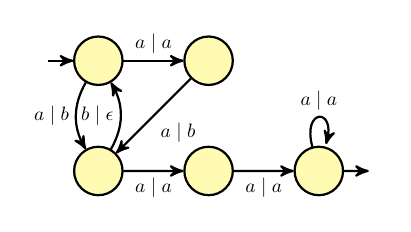
\begin{tikzpicture}[->,>=stealth',auto,node distance=2cm,thick,scale=0.7,every node/.style={scale=0.7}]
  \tikzstyle{every state}=[fill=yellow!30,text=black]
\tikzstyle{initial}=[initial by arrow, initial where=left, initial text=]
  \tikzstyle{accepting}=[accepting by arrow, accepting where=right, accepting text=]

  \node[initial,state] (A)  {};
  \node[state] [right of=A] (B)  {};
  \node[state] [below of=A] (C)  {};
  \node[state] [right of=C] (D)  {};
  \node[accepting,state] [right of=D] (E)  {};
  \path (A) edge node {\trans{a}{a}} (B);
  \path (A) edge [bend right,left] node {\trans{a}{b}} (C);
  \path (B) edge node {\trans{a}{b}} (C);
  \path (C) edge [bend right] node  {\trans{b}{\epsilon}} (A);
  \path (C) edge [below] node {\trans{a}{a}} (D);
  \path (D) edge [below] node {\trans{a}{a}} (E);
  \path (E) edge [loop above] node {\trans{a}{a}} (E);
\end{tikzpicture}
}
\subfigure[\label{exmultnseq-det}]{
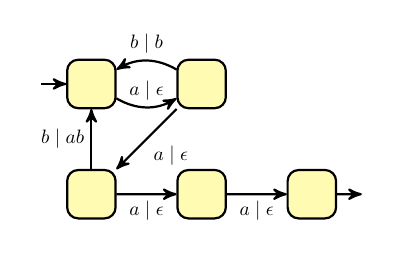
\begin{tikzpicture}[->,>=stealth',auto,node distance=2cm,thick,scale=0.7,every node/.style={scale=0.7}]
  \tikzstyle{every state}=[fill=yellow!30,text=black, shape = rectangle,rounded corners,font=\scriptsize]
\tikzstyle{initial}=[initial by arrow, initial where=left, initial text=]
  \tikzstyle{accepting}=[accepting by arrow, accepting where=right, accepting text=]

  \node[initial,state] (A)  {};
  \node[state] [right of=A] (B)  {};
  \node[state] [below of=A] (C)  {};
  \node[state] [right of=C] (D)  {};
  \node[state,accepting] [right of=D] (E)  {};
  \path (A) edge [bend right] node {\trans{a}{\epsilon}} (B);
  \path (B) edge node {\trans{a}{\epsilon}} (C);
  \path (C) edge [below] node {\trans{a}{\epsilon}} (D);
  \path (B) edge [bend right,above] node {\trans{b}{b}} (A);
  \path (C) edge node {\trans{b}{ab}} (A);
  \path (D) edge [below] node {\trans{a}{\epsilon}} (E);
\end{tikzpicture}
}
\vspace{-4mm}
\caption{\label{fig:det1} Non determinisable transducer.}
\vspace{-6mm}
\end{figure}

\paragraph{\textbf{Weak determinisation}} Let  be a trim transducer with a single initial state.
For every , let the rank 
of  be the set containing all the SCC of  accessible from the
states . The multi-transducer  is obtained from  by splitting the edges that do not preserve the rank, as follows.
If  is an edge of  such that
 is strictly included in , it is removed, and replaced
by the set of edges . It is easily shown that any pair of distinct edges of the form 
 and  in  have necessarily been
created by this transformation (because without this transformation
everything stays input-deterministic). Therefore, since the rank
strictly decreases ( and ) and can never increase in , there is no
run from  to , nor from  to  in
, and the two edges are transient. As a
consequence, 

\begin{lemma}\label{lem:separable}
The infinite transducer  is separable.
\end{lemma}


The weak determinisation of , written , is the trim part of .


\begin{proposition}\label{weakdet}
 and  are equivalent. Moreover, 
if  is weakly twinned,  is finite, and it
is a multi-transducer.
\end{proposition}

The main idea is to prove that, as long as the weak twinning property
is satisfied, the length of the words present in the states of
 can be bounded. The proof can be found in
Appendix. 


\begin{example}
Let us illustrate the weak determinisation on the transducer  of
Fig.~\ref{exmultnseq}. Consider the determinisation
 of  of Fig.~\ref{exmultnseq-det}.
When it is in state , on input , it moves to
state , definitely leaving the SCC
 of  (the rank  of  is
strictly included in the rank  of ). As a result, this
transition is removed from , and replaced by the
transitions  and
. The resulting transducer
 is depicted on Fig.~\ref{fig:wdet1} (where the new
transitions are dotted). Fig.~\ref{fig:split_wdet1} shows how the
latter transducer is split into a union.
\end{example}




\paragraph{Proof of Lemma \ref{lem:decomposition}} We can finally prove that the every weakly twinned transducer is multi-sequential.
Let  be a weakly twinned transducer.
Then  is equivalent to , where  is the transducer obtained by keeping only  as initial state.
Given , as we just saw,  is a transducer equivalent to .
Moreover, as  is separable, so is ,hence, by Lemma , it is multi-sequential.
The desired result follows.



\begin{figure}[!ht]
\subfigure[\label{fig:wdet1}]{
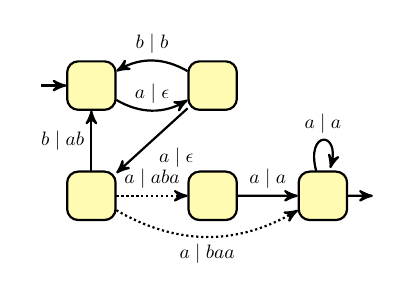
\begin{tikzpicture}[->,>=stealth',auto,node distance=2cm,thick,scale=0.7,every node/.style={scale=0.7}]
  \tikzstyle{every state}=[fill=yellow!30,text=black, shape = rectangle,rounded corners,font=\scriptsize]
\tikzstyle{initial}=[initial by arrow, initial where=left, initial text=]
  \tikzstyle{accepting}=[accepting by arrow, accepting where=right, accepting text=]

  \node[initial,state] (A) at (0,0) {};
  \node[state] (B) at (2.2,0) {};
  \node[state] [below of=A] (C)  {};
  \node[state] (D) at (2.2,-2) {};
  \node[state,accepting] [right of=D] (E)  {};
  \path (A) edge [bend right] node {\trans{a}{\epsilon}} (B);
  \path (B) edge node {\trans{a}{\epsilon}} (C);
  \path (C) edge [densely dotted] node {\trans{a}{aba}} (D);
  \path (C) edge [bend right,below,densely dotted] node {\trans{a}{baa}} (E);
  \path (B) edge [bend right,above] node {\trans{b}{b}} (A);
  \path (C) edge node {\trans{b}{ab}} (A);
  \path (D) edge node {\trans{a}{a}} (E);
  \path (E) edge [loop above] node {\trans{a}{a}} (E);
\end{tikzpicture}
}
\subfigure[\label{fig:split_wdet1}]{
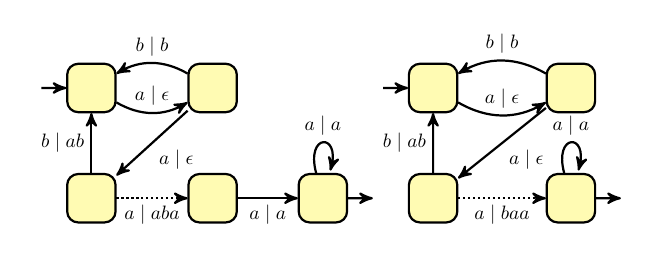
\begin{tikzpicture}[->,>=stealth',auto,node distance=2cm,thick,scale=0.7,every node/.style={scale=0.7}]
  \tikzstyle{every state}=[fill=yellow!30,text=black, shape = rectangle,rounded corners]
\tikzstyle{initial}=[initial by arrow, initial where=left, initial text=]
  \tikzstyle{accepting}=[accepting by arrow, accepting where=right, accepting text=]



  \node[initial,state] (A) at (0,1) {};
  \node[state] (B) at (2.2,1) {};
  \node[state] (C) at (0,-1) {};
  \node[state] (D) at (2.2,-1) {};
  \node[state,accepting] (E) at (4.2,-1)  {};
  \path (A) edge [bend right] node {\trans{a}{\epsilon}} (B);
  \path (B) edge node {\trans{a}{\epsilon}} (C);
  \path (C) edge [densely dotted] node [below] {\trans{a}{aba}} (D);
  \path (B) edge [above,bend right] node {\trans{b}{b}} (A);
  \path (C) edge node {\trans{b}{ab}} (A);
  \path (D) edge node [below] {\trans{a}{a}} (E);
  \path (E) edge [loop above] node {\trans{a}{a}} (E);



  \node[initial,state] (A') at (6.2,1)  {};
  \node[state] (B') at (8.7,1) {};
  \node[state] (C') at (6.2,-1)  {};
\node[state,accepting] (E') at (8.7,-1) {};
  \path (A') edge [bend right] node {\trans{a}{\epsilon}} (B');
  \path (B') edge node {\trans{a}{\epsilon}} (C');
  \path (C') edge [densely dotted] node [below] {\trans{a}{baa}} (E');
  \path (B') edge [above,bend right] node {\trans{b}{b}} (A');
  \path (C') edge node {\trans{b}{ab}} (A');
  \path (E') edge [loop above] node {\trans{a}{a}} (E');
\end{tikzpicture}
}
\vspace{-4mm}
\caption{Weak determinisation and split}
\vspace{-8mm}
\end{figure}




\section{Application to Multi-Output Streamability Problem}

Sequential functions have the advantage of being efficiently
computable. They are exactly the word functions that can be evaluated
with constant memory in a sequential, left-to-right, manner. This
computability notion have been defined formally in
\cite{DBLP:conf/fsttcs/FiliotGRS11} with the model of Turing
transducers. Informally, a Turing transducer has three tapes: a
read-only left-to-right input tape, a working tape, and a write-only
left-to-right output tape. The amount of memory is measured only on
the working tape. For any sequential function , there exists a
Turing transducer  and constant  such that for all words ,  can be computed by  while using at most  cells of
the working tape. This model is a streaming model in the sense that 
the input tape is left-to-right, and therefore one can think of
receiving the input word  as a stream. The converse also holds
true: any word function computable with constant memory by a Turing
transducer is sequential. Therefore, the following problem, called the
streamability problem, is decidable in \textsc{PTime}, based on the
twinning property: given a functional transducer, does it define a
function that can be evaluated with constant memory? In this section,
we establish a similar result for relations. 


We extend the model of Turing transducer to a model for computing
relations. We rather explain this model in words, avoiding a tedious
and technical definition of intuitive concepts. This model can be thought of as a streaming model where the input
word  is a stream, and the outputs words are produced on-the-fly, while
processing , and sent through different channels (represented as
output tapes in the model). More precisely, let . 
A \emph{-output Turing
transducer}  is a deterministic Turing machine with  a read-only
left-to-right input tape,  a two-way working tape, and  
write-only left-to-right output tapes without stay
transitions (therefore a cell cannot be rewritten). Additionally, the
machine can disable/enable some output tapes. A \emph{tape
  configuration} of such a machine is a tuple  where  is
the content of the input tape,  is the content of the working tape,
and  is the set of contents of the enabled output tapes. By content we mean the sequence of
symbols to the first blank symbol.



To define the class of constant memory computable relations, we will
allow some preprocessing of the input stream, i.e., the computation of 
a constant amount of information that can be then exploited by the
machine to compute the output words. In the setting of sequential
function, this information is implicitly present in the definition of
constant memory computability: it is assumed that the input stream belongs to the domain
of the function, otherwise it could start producing some output word
and realise later on that the word was not in the domain. The
information of being in the domain or not (a 0/1 bit) is typically some
preprocessing computation that can be performed on the input word, by
some other application. For instance, if the stream is generated by
another application, this application could also send the information
on whether the stream belong to the domain of the function or not. 


We come to the definition of constant memory computability for
relations. Let . We say that  is \emph{constant memory computable} if
there exist two constants , a
computable function  such that for
all , , and a -output Turing transducer  over the alphabet \}\q_1 \xrightarrow{u\mid u_1} q_1 \xrightarrow{v\mid v_1} q_1 \xrightarrow{u\mid u_2} q_2 \xrightarrow{v\mid v_2} q_2q_1 \xrightarrow{u\mid u_1} q_1 \xrightarrow{v\mid v_1} q_1 \xrightarrow{u\mid u_2} q_2 \xrightarrow{v\mid v_2} q_2\delay(u_1v_1,u_2v_2) = \delay(u_1v_1,u_1v_1^{k+1}v_1') = \delay(\epsilon,v_1^{k}v_1') = \delay(u_1,u_1v_1^{k}v_1') = \delay(u_1,u_2),q_1 \xrightarrow{uv^n\mid  u_1v_1^n} q_1 \xrightarrow{v\mid v_1} q_1 \xrightarrow{uv^n\mid u_2v_2^n} q_2 \xrightarrow{v\mid v_2} q_2q_1 \xrightarrow{u\mid u_1} q_1 \xrightarrow{v\mid v_1} q_1 \xrightarrow{u\mid u_2} q_2 \xrightarrow{v\mid v_2} q_2q_1 \xrightarrow{u\mid u_1} q_1 \xrightarrow{v\mid v_1} q_1 \xrightarrow{u\mid u_2} q_2 \xrightarrow{v\mid v_2} q_2q_1 \xrightarrow{u\mid u_1} q_1 \xrightarrow{uv^{|u_1| - |u_2|} \mid u_1v_1^{|u_1| - |u_2|}} q_1 \xrightarrow{uv^{|u_1| - |u_2|}\mid u_2v_2^{|u_1| - |u_2|}} q_2 \xrightarrow{v\mid v_2} q_2,\begin{array}{lcl}
p_1 & : &  \bar{q} \xrightarrow{\textsf{p}(u_1,u_2)|v} q \xrightarrow{\textsf{d}(u_1,u_2)|v_1''} q_1,\\
p_2 & : & \bar{q} \xrightarrow{\textsf{p}(u_1,u_2)|v} q \xrightarrow{\textsf{d}(u_2,u_1)|v_2''} q_2.
\end{array}\begin{array}{lcl}
|\Delta(v_1,v_2)| & = & |\textsf{d}(v_1,v_2)| + |\textsf{d}(v_2,v_1)|\\
& = & |v_1| + |v_2| - 2|\textsf{p}(v_1,v_2)|\\
& = & 2 |v| + |v_1''| + |v_2''| + |f_T(q_1)| + |f_T(q_2)| - 2|\textsf{p}(v_1,v_2)|\\
& \leq & |v_1''| + |v_2''| + |f_T(q_1)| + |f_T(q_2)|\\
& \leq & M_{\mathcal{D}} |\textsf{d}(u_1,u_2)| + M_{\mathcal{D}} |\textsf{d}(u_2,u_1)| + 2 M_{\mathcal{D}}\\
& = & M_{\mathcal{D}} (|\Delta(u_1,u_2)|+2).
\end{array}
q_1\xrightarrow{u|u_1} q_1\xrightarrow{v|v_1}q_1\xrightarrow{u|u_2} q_2\xrightarrow{v|v_2} q_2
\begin{array}{ll}
R_{U,v} & = \{(q,w) \in Q \times \Gamma^* | \exists (p,u) \in U,v'\in \Gamma^* \textup{ s.t. } p \xrightarrow{v|v'}_{\tra} q \textup{ and } w = uv'\},\\
w_{U,v} & \textup{be the largest common prefix of the words } \} ,\\
P_{U,v} & = \{(q,w) | (q,w_{U,v}w) \in R_{U,v} \}.
\end{array}U \xrightarrow{v_0|w_{U,v_0}} P_{U,v_0}.P_{U,v_0} \xrightarrow{\sigma|w_{P_{U,v_0},\sigma}} P_{P_{U,v_0},\sigma}.U \xrightarrow{v|w_{U,v_0}w_{P_{U,v_0},\sigma}} P_{P_{U,v_0},\sigma}.\begin{array}{lcl}
(u,v) \in \inter{\tra} & \Leftrightarrow & \textup{there exists an accepting run } q_0 \xrightarrow{u|w}_{\tra} q \textup{ s.t. } v = wf_T(q)\\
& \Leftrightarrow & \exists q \in T, \exists w \in \Gamma^* \textup{ s.t. } (q,w) \in R_{U_0,u} \textup{ and }v = wf_T(q)\\
& \Leftrightarrow & \exists q \in T, \exists w' \in \Gamma^* \textup{ s.t. } (q,w) \in P_{U_0,u} \textup{ and }v = w_{U_0,u}w'f_T(q)\\
& \Leftrightarrow & (u,v) \in \inter{\mathcal{D}(\tra)}\\
\end{array}\{ (q,w_{U,v}w) | (q,w) \in P_{U,v} \} = \bigcup_{(q,w) \in U} \{ (q',ww_{\{ (q,\epsilon)\},v}w') | (q',w') \in P_{\{ (q,\epsilon)\},v} \},\begin{array}{lll}
r_0 & : & p = p_0^0 \xrightarrow{u^1|v_0^1} p_0^1 \xrightarrow{u^2|v_0^2} \ldots \xrightarrow{u^n|v_0^{n}} p_0^{n} = p_0,\\
r_1 & : & p = p_1^0 \xrightarrow{u^1|v_1^1} p_1^1 \xrightarrow{u^2|v_1^2} \ldots \xrightarrow{u^n|v_1^{n}} p_1^{n} = p_1,\\
r_2 & : & p = p_2^0 \xrightarrow{u^1|v_2^1} p_2^1 \xrightarrow{u^2|v_2^2} \ldots \xrightarrow{u^n|v_2^{n}} p_2^{n} = p_2,
\end{array}\Delta(v_1^{1} \ldots v_1^{i_1}v_1^{i_2} \ldots v_1^{n},v_2^{1} \ldots v_2^{i_1}v_2^{i_2} \ldots v_2^{n}) = \Delta(v_1^{1} \ldots v_1^{n},v_2^{1} \ldots v_2^{n}) \geq  2M_{\tra} |Q|^3,\begin{array}{llll}
p_0 \xrightarrow{x_0|y_0} p \xrightarrow{u^{1} \ldots u^{i_1}|v_j^{1} \ldots v_j^{i_1}} p_j^{i_1}, & \ & p_0^{i_1}  \xrightarrow{u^{i_1} \ldots u^{i_2}|v_0^{i_1} \ldots v_0^{i_2}} p_0^{i_1},\\
p_0 \xrightarrow{x_0|y_0} p \xrightarrow{u^{1} \ldots u^{i_1}|v_0^{1} \ldots v_0^{i_1}} p_0^{i_1}, & \ & p_j^{i_1} \xrightarrow{u^{i_1} \ldots u^{i_2}|v_j^{i_1} \ldots v_j^{i_2}} p_j^{i_1}.
\end{array}\begin{array}{lllll}
q_0 & \xrightarrow{aaaa|a} & q_5 & \xrightarrow{ba|a} & q_5,\\
q_0 & \xrightarrow{aaaa|b} & q_5 & \xrightarrow{ba|a} & q_5.
\end{array}\begin{array}{lllll}
q_0 & \xrightarrow{aaaaa|baaaa} & q_6 & \xrightarrow{a|a} & q_6,\\
q_0 & \xrightarrow{aaaaa|abaaa} & q_6 & \xrightarrow{a|a} & q_6.
\end{array}
Therefore, the determinisation is infinite.
However, the weak determinisation is finite.
The dotted edge of , definitely leaving the SCC  of , is split into the three dotted edges of .
The figure  exposes the decomposition of  into a union of sequential transducers.\\ 

\begin{figure}[!ht]
\subfigure[\label{ex21}]{
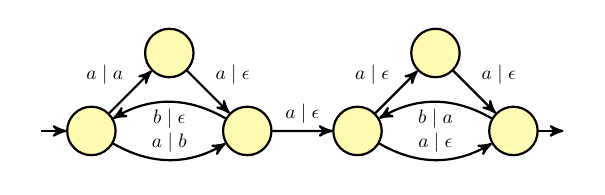
\begin{tikzpicture}[->,>=stealth',auto,node distance=2cm,thick,scale=0.7,every node/.style={scale=0.7}]
  \tikzstyle{every state}=[fill=yellow!30,text=black]
\tikzstyle{initial}=[initial by arrow, initial where=left, initial text=]
  \tikzstyle{accepting}=[accepting by arrow, accepting where=right, accepting text=]

  \node[initial,state] (A)  {};
  \node[state] [above right of=A] (B)  {};
  \node[state] [below right of=B] (C)  {};
  \node[state] [right of=C] (D)  {};
  \node[state] [above right of=D] (E)  {};
  \node[accepting,state] [below right of=E] (F)  {};
  \path (A) edge node {\trans{a}{a}} (B);
  \path (B) edge node {\trans{a}{\epsilon}} (C);
  \path (A) edge [bend right] node {\trans{a}{b}} (C);
  \path (C) edge [bend right] node {\trans{b}{\epsilon}} (A);
  \path (C) edge node {\trans{a}{\epsilon}} (D);
  \path (D) edge node {\trans{a}{\epsilon}} (E);
  \path (D) edge [bend right] node {\trans{a}{\epsilon}} (F);
  \path (E) edge node {\trans{a}{\epsilon}} (F);
  \path (F) edge [bend right] node {\trans{b}{a}} (D);
\end{tikzpicture}
}

\subfigure[\label{ex22}]{
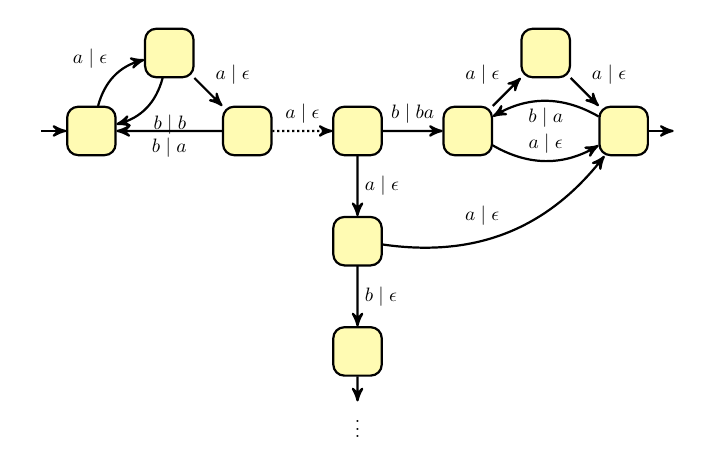
\begin{tikzpicture}[->,>=stealth',auto,node distance=2cm,thick,scale=0.7,every node/.style={scale=0.7}]
  \tikzstyle{every state}=[fill=yellow!30,text=black, shape = rectangle,rounded corners]
\tikzstyle{initial}=[initial by arrow, initial where=left, initial text=]
  \tikzstyle{accepting}=[accepting by arrow, accepting where=right, accepting text=]

  \node[initial,state] (A)  {};
  \node[state] [above right of=A] (B)  {};
  \node[state] [below right of=B] (C)  {};
  \node[state] [right of=C] (D)  {};
  \node[state] [right of=D] (D1)  {};
  \node[state] [above right of=D1] (D2)  {};
  \node[accepting,state] [below right of=D2] (D3)  {};
  \node[state] [below of=D] (E)  {};


  \tikzstyle{accepting}=[accepting by arrow, accepting where=below, accepting text=\vdots]


  \node[accepting,state] [below of=E] (F)  {};
  \path (B) edge node {\trans{a}{\epsilon}} (C);
  \path (A) edge [bend left] node {\trans{a}{\epsilon}} (B);
  \path (B) edge [bend left] node {\trans{b}{b}} (A);
  \path (C) edge node {\trans{b}{a}} (A);
  \path (C) edge [densely dotted] node {\trans{a}{\epsilon}} (D);
  \path (D) edge node {\trans{b}{ba}} (D1);
  \path (D1) edge node {\trans{a}{\epsilon}} (D2);
  \path (D1) edge [bend right] node {\trans{a}{\epsilon}} (D3);
  \path (D2) edge node {\trans{a}{\epsilon}} (D3);
  \path (D3) edge [bend right] node {\trans{b}{a}} (D1);
  \path (D) edge node {\trans{a}{\epsilon}} (E);
  \path (E) edge [bend right] node {\trans{a}{\epsilon}} (D3);
  \path (E) edge node {\trans{b}{\epsilon}} (F);
\end{tikzpicture}
}

\subfigure[\label{ex23}]{
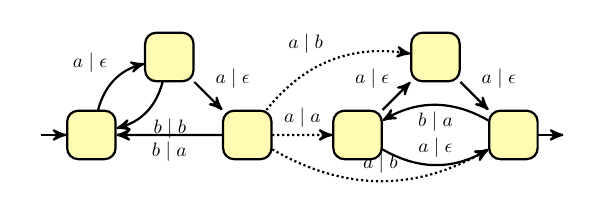
\begin{tikzpicture}[->,>=stealth',auto,node distance=2cm,thick,scale=0.7,every node/.style={scale=0.7}]
  \tikzstyle{every state}=[fill=yellow!30,text=black, shape = rectangle,rounded corners]
\tikzstyle{initial}=[initial by arrow, initial where=left, initial text=]
  \tikzstyle{accepting}=[accepting by arrow, accepting where=right, accepting text=]

  \node[initial,state] (A)  {};
  \node[state] [above right of=A] (B)  {};
  \node[state] [below right of=B] (C)  {};
  \node[state] [right of=C] (D)  {};
  \node[state] [above right of=D] (E)  {};
  \node[state,accepting] [below right of=E] (F)  {};
  \path (B) edge node {\trans{a}{\epsilon}} (C);
  \path (A) edge [bend left] node {\trans{a}{\epsilon}} (B);
  \path (B) edge [bend left] node {\trans{b}{b}} (A);
  \path (C) edge node {\trans{b}{a}} (A);
  \path (C) edge [densely dotted] node {\trans{a}{a}} (D);
  \path (C) edge [densely dotted, bend left] node {\trans{a}{b}} (E);
  \path (C) edge [densely dotted, bend right] node {\trans{a}{b}} (F);
  \path (D) edge node {\trans{a}{\epsilon}} (E);
  \path (D) edge [bend right] node {\trans{a}{\epsilon}} (F);
  \path (E) edge node {\trans{a}{\epsilon}} (F);
  \path (F) edge [bend right] node {\trans{b}{a}} (D);
\end{tikzpicture}
}
\caption{Multisequential transducer that is not sequential.}
\label{fig:det2} 
\end{figure}


\begin{figure}[!ht]
\subfigure{
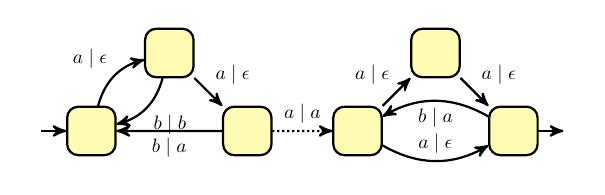
\begin{tikzpicture}[->,>=stealth',auto,node distance=2cm,thick,scale=0.7,every node/.style={scale=0.7}]
  \tikzstyle{every state}=[fill=yellow!30,text=black, shape = rectangle,rounded corners]
\tikzstyle{initial}=[initial by arrow, initial where=left, initial text=]
  \tikzstyle{accepting}=[accepting by arrow, accepting where=right, accepting text=]

  \node[initial,state] (A)  {};
  \node[state] [above right of=A] (B)  {};
  \node[state] [below right of=B] (C)  {};
  \node[state] [right of=C] (D)  {};
  \node[state] [above right of=D] (E)  {};
  \node[state,accepting] [below right of=E] (F)  {};
  \path (B) edge node {\trans{a}{\epsilon}} (C);
  \path (A) edge [bend left] node {\trans{a}{\epsilon}} (B);
  \path (B) edge [bend left] node {\trans{b}{b}} (A);
  \path (C) edge node {\trans{b}{a}} (A);
  \path (C) edge [densely dotted] node {\trans{a}{a}} (D);
  \path (D) edge node {\trans{a}{\epsilon}} (E);
  \path (D) edge [bend right] node {\trans{a}{\epsilon}} (F);
  \path (E) edge node {\trans{a}{\epsilon}} (F);
  \path (F) edge [bend right] node {\trans{b}{a}} (D);
\end{tikzpicture}
}

\subfigure{
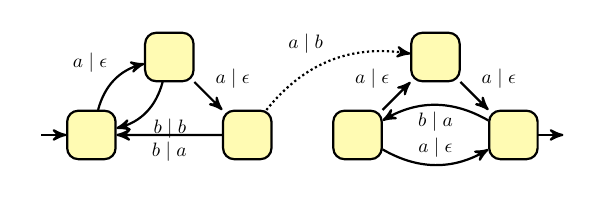
\begin{tikzpicture}[->,>=stealth',auto,node distance=2cm,thick,scale=0.7,every node/.style={scale=0.7}]
  \tikzstyle{every state}=[fill=yellow!30,text=black, shape = rectangle,rounded corners]
\tikzstyle{initial}=[initial by arrow, initial where=left, initial text=]
  \tikzstyle{accepting}=[accepting by arrow, accepting where=right, accepting text=]

  \node[initial,state] (A)  {};
  \node[state] [above right of=A] (B)  {};
  \node[state] [below right of=B] (C)  {};
  \node[state] [right of=C] (D)  {};
  \node[state] [above right of=D] (E)  {};
  \node[state,accepting] [below right of=E] (F)  {};
  \path (B) edge node {\trans{a}{\epsilon}} (C);
  \path (A) edge [bend left] node {\trans{a}{\epsilon}} (B);
  \path (B) edge [bend left] node {\trans{b}{b}} (A);
  \path (C) edge node {\trans{b}{a}} (A);
  \path (C) edge [densely dotted, bend left] node {\trans{a}{b}} (E);
  \path (D) edge node {\trans{a}{\epsilon}} (E);
  \path (D) edge [bend right] node {\trans{a}{\epsilon}} (F);
  \path (E) edge node {\trans{a}{\epsilon}} (F);
  \path (F) edge [bend right] node {\trans{b}{a}} (D);
\end{tikzpicture}
}

\subfigure{
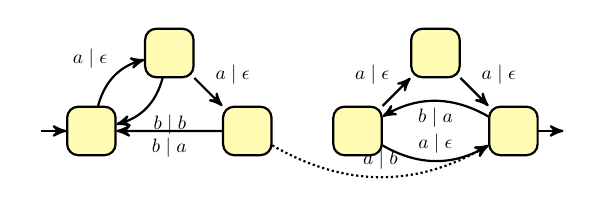
\begin{tikzpicture}[->,>=stealth',auto,node distance=2cm,thick,scale=0.7,every node/.style={scale=0.7}]
  \tikzstyle{every state}=[fill=yellow!30,text=black, shape = rectangle,rounded corners]
\tikzstyle{initial}=[initial by arrow, initial where=left, initial text=]
  \tikzstyle{accepting}=[accepting by arrow, accepting where=right, accepting text=]

  \node[initial,state] (A)  {};
  \node[state] [above right of=A] (B)  {};
  \node[state] [below right of=B] (C)  {};
  \node[state] [right of=C] (D)  {};
  \node[state] [above right of=D] (E)  {};
  \node[state,accepting] [below right of=E] (F)  {};
  \path (B) edge node {\trans{a}{\epsilon}} (C);
  \path (A) edge [bend left] node {\trans{a}{\epsilon}} (B);
  \path (B) edge [bend left] node {\trans{b}{b}} (A);
  \path (C) edge node {\trans{b}{a}} (A);
  \path (C) edge [densely dotted, bend right] node {\trans{a}{b}} (F);
  \path (D) edge node {\trans{a}{\epsilon}} (E);
  \path (D) edge [bend right] node {\trans{a}{\epsilon}} (F);
  \path (E) edge node {\trans{a}{\epsilon}} (F);
  \path (F) edge [bend right] node {\trans{b}{a}} (D);
\end{tikzpicture}
}
\caption{The transducer }
\label{fig:det2b} 
\end{figure}

\begin{figure}[!ht]
\subfigure[\label{ex31}]{
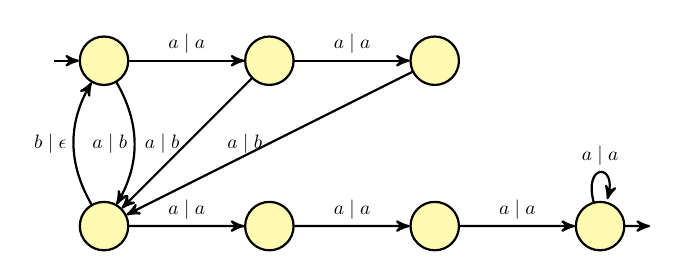
\begin{tikzpicture}[->,>=stealth',auto,node distance=3cm,thick,scale=0.7,every node/.style={scale=0.7}]
  \tikzstyle{every state}=[fill=yellow!30,text=black]
\tikzstyle{initial}=[initial by arrow, initial where=left, initial text=]
  \tikzstyle{accepting}=[accepting by arrow, accepting where=right, accepting text=]

  \node[initial,state] (A)  {};
  \node[state] [right of=A] (B)  {};
  \node[state] [right of=B] (C)  {};
  \node[state] [below of=A] (D)  {};
  \node[state] [right of=D] (E)  {};
  \node[state] [right of=E] (F)  {};
  \node[accepting,state] [right of=F] (G)  {};
  \path (A) edge node {\trans{a}{a}} (B);
  \path (B) edge node {\trans{a}{a}} (C);
  \path (A) edge [left, bend left] node {\trans{a}{b}} (D);
  \path (B) edge [left] node {\trans{a}{b}} (D);
  \path (C) edge [left] node {\trans{a}{b}} (D);
  \path (D) edge [left, bend left] node {\trans{b}{\epsilon}} (A);
  \path (D) edge node {\trans{a}{a}} (E);
  \path (E) edge node {\trans{a}{a}} (F);
  \path (F) edge node {\trans{a}{a}} (G);
  \path (G) edge [loop above] node {\trans{a}{a}} (G);
\end{tikzpicture}
}

\subfigure[\label{ex32}]{
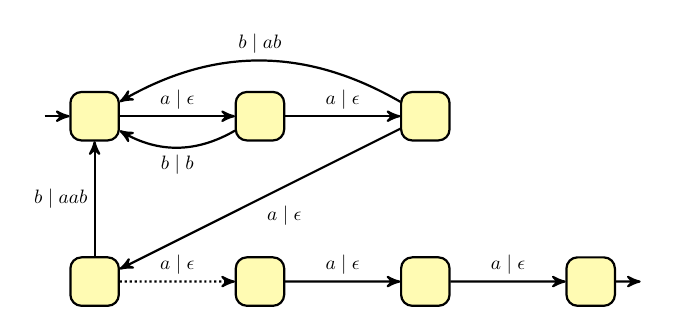
\begin{tikzpicture}[->,>=stealth',auto,node distance=3cm,thick,scale=0.7,every node/.style={scale=0.7}]
  \tikzstyle{every state}=[fill=yellow!30,text=black, shape = rectangle,rounded corners]
\tikzstyle{initial}=[initial by arrow, initial where=left, initial text=]
  \tikzstyle{accepting}=[accepting by arrow, accepting where=right, accepting text=]

  \node[initial,state] (A)  {};
  \node[state] [right of=A] (B)  {};
  \node[state] [right of=B] (C)  {};
  \node[state] [below of=A] (D)  {};
  \node[state] [right of=D] (E)  {};
  \node[state] [right of=E] (F)  {};
  \node[accepting,state] [right of=F] (G)  {};
  \path (A) edge node {\trans{a}{\epsilon}} (B);
  \path (B) edge node {\trans{a}{\epsilon}} (C);
  \path (C) edge node {\trans{a}{\epsilon}} (D);
  \path (B) edge [bend left] node {\trans{b}{b}} (A);
  \path (C) edge [above,bend right] node {\trans{b}{ab}} (A);
  \path (D) edge node {\trans{b}{aab}} (A);
  \path (D) edge [densely dotted] node {\trans{a}{\epsilon}} (E);
  \path (E) edge node {\trans{a}{\epsilon}} (F);
  \path (F) edge node {\trans{a}{\epsilon}} (G);
\end{tikzpicture}
}

\subfigure[\label{ex33}]{
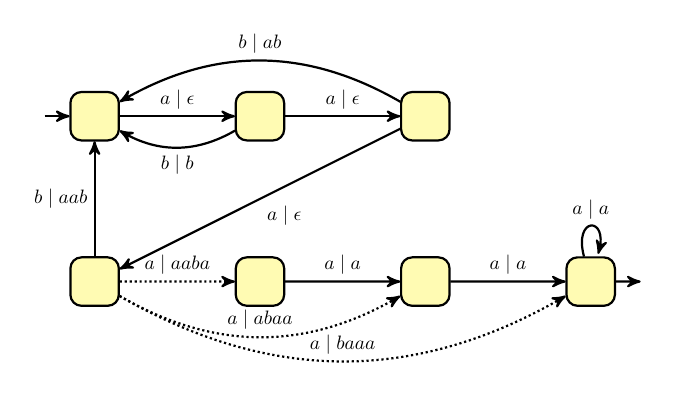
\begin{tikzpicture}[->,>=stealth',auto,node distance=3cm,thick,scale=0.7,every node/.style={scale=0.7}]
  \tikzstyle{every state}=[fill=yellow!30,text=black, shape = rectangle,rounded corners]
\tikzstyle{initial}=[initial by arrow, initial where=left, initial text=]
  \tikzstyle{accepting}=[accepting by arrow, accepting where=right, accepting text=]

  \node[initial,state] (A)  {};
  \node[state] [right of=A] (B)  {};
  \node[state] [right of=B] (C)  {};
  \node[state] [below of=A] (D)  {};
  \node[state] [right of=D] (E)  {};
  \node[state] [right of=E] (F)  {};
  \node[accepting,state] [right of=F] (G)  {};
  \path (A) edge node {\trans{a}{\epsilon}} (B);
  \path (B) edge node {\trans{a}{\epsilon}} (C);
  \path (C) edge node {\trans{a}{\epsilon}} (D);
  \path (B) edge [bend left] node {\trans{b}{b}} (A);
  \path (C) edge [above,bend right] node {\trans{b}{ab}} (A);
  \path (D) edge node {\trans{b}{aab}} (A);
  \path (D) edge [densely dotted] node {\trans{a}{aaba}} (E);
  \path (D) edge [densely dotted, bend right] node {\trans{a}{abaa}} (F);
  \path (D) edge [densely dotted, bend right] node {\trans{a}{baaa}} (G);
  \path (E) edge node {\trans{a}{a}} (F);
  \path (F) edge node {\trans{a}{a}} (G);
  \path (G) edge [loop above] node {\trans{a}{a}} (G);
\end{tikzpicture}
}
\caption{Multisequential transducer that is not sequential.}
\label{fig:det3} 
\end{figure}

\begin{figure}[!ht]
\subfigure{
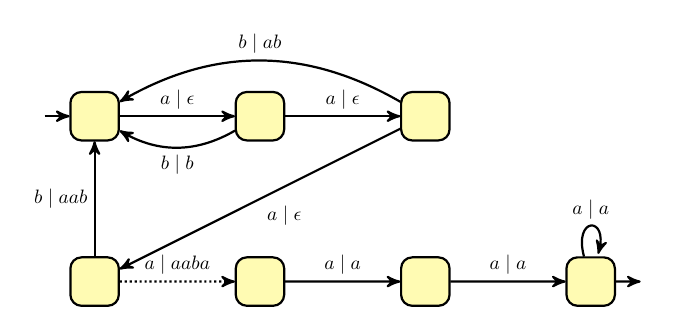
\begin{tikzpicture}[->,>=stealth',auto,node distance=3cm,thick,scale=0.7,every node/.style={scale=0.7}]
  \tikzstyle{every state}=[fill=yellow!30,text=black, shape = rectangle,rounded corners]
\tikzstyle{initial}=[initial by arrow, initial where=left, initial text=]
  \tikzstyle{accepting}=[accepting by arrow, accepting where=right, accepting text=]

  \node[initial,state] (A)  {};
  \node[state] [right of=A] (B)  {};
  \node[state] [right of=B] (C)  {};
  \node[state] [below of=A] (D)  {};
  \node[state] [right of=D] (E)  {};
  \node[state] [right of=E] (F)  {};
  \node[accepting,state] [right of=F] (G)  {};
  \path (A) edge node {\trans{a}{\epsilon}} (B);
  \path (B) edge node {\trans{a}{\epsilon}} (C);
  \path (C) edge node {\trans{a}{\epsilon}} (D);
  \path (B) edge [bend left] node {\trans{b}{b}} (A);
  \path (C) edge [above, bend right] node {\trans{b}{ab}} (A);
  \path (D) edge node {\trans{b}{aab}} (A);
  \path (D) edge [densely dotted] node {\trans{a}{aaba}} (E);
  \path (E) edge node {\trans{a}{a}} (F);
  \path (F) edge node {\trans{a}{a}} (G);
  \path (G) edge [loop above] node {\trans{a}{a}} (G);
\end{tikzpicture}
}

\subfigure{
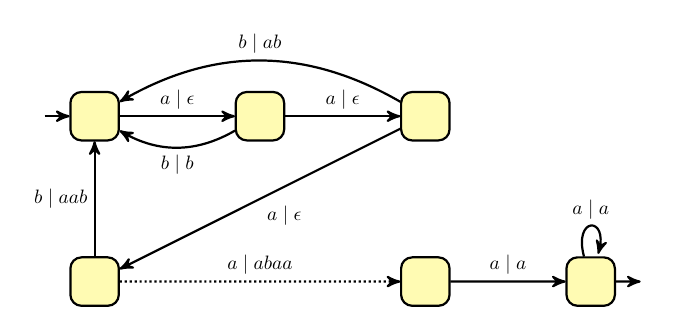
\begin{tikzpicture}[->,>=stealth',auto,node distance=3cm,thick,scale=0.7,every node/.style={scale=0.7}]
  \tikzstyle{every state}=[fill=yellow!30,text=black, shape = rectangle,rounded corners]
\tikzstyle{initial}=[initial by arrow, initial where=left, initial text=]
  \tikzstyle{accepting}=[accepting by arrow, accepting where=right, accepting text=]

  \node[initial,state] (A)  {};
  \node[state] [right of=A] (B)  {};
  \node[state] [right of=B] (C)  {};
  \node[state] [below of=A] (D)  {};
  \node [right of=D] (E)  {};
  \node[state] [right of=E] (F)  {};
  \node[accepting,state] [right of=F] (G)  {};
  \path (A) edge node {\trans{a}{\epsilon}} (B);
  \path (B) edge node {\trans{a}{\epsilon}} (C);
  \path (C) edge node {\trans{a}{\epsilon}} (D);
  \path (B) edge [bend left] node {\trans{b}{b}} (A);
  \path (C) edge [above, bend right] node {\trans{b}{ab}} (A);
  \path (D) edge node {\trans{b}{aab}} (A);
  \path (D) edge [densely dotted] node {\trans{a}{abaa}} (F);
  \path (F) edge node {\trans{a}{a}} (G);
  \path (G) edge [loop above] node {\trans{a}{a}} (G);
\end{tikzpicture}
}

\subfigure{
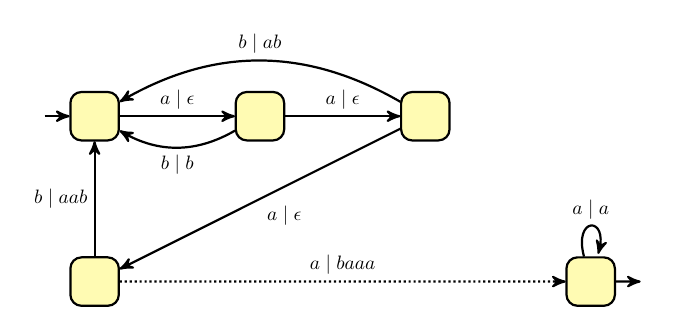
\begin{tikzpicture}[->,>=stealth',auto,node distance=3cm,thick,scale=0.7,every node/.style={scale=0.7}]
  \tikzstyle{every state}=[fill=yellow!30,text=black, shape = rectangle,rounded corners]
\tikzstyle{initial}=[initial by arrow, initial where=left, initial text=]
  \tikzstyle{accepting}=[accepting by arrow, accepting where=right, accepting text=]

  \node[initial,state] (A)  {};
  \node[state] [right of=A] (B)  {};
  \node[state] [right of=B] (C)  {};
  \node[state] [below of=A] (D)  {};
  \node [right of=D] (E)  {};
  \node [right of=E] (F)  {};
  \node[accepting,state] [right of=F] (G)  {};
  \path (A) edge node {\trans{a}{\epsilon}} (B);
  \path (B) edge node {\trans{a}{\epsilon}} (C);
  \path (C) edge node {\trans{a}{\epsilon}} (D);
  \path (B) edge [bend left] node {\trans{b}{b}} (A);
  \path (C) edge [above, bend right] node {\trans{b}{ab}} (A);
  \path (D) edge node {\trans{b}{aab}} (A);
  \path (D) edge [densely dotted] node {\trans{a}{baaa}} (G);
  \path (G) edge [loop above] node {\trans{a}{a}} (G);
\end{tikzpicture}
}
\caption{The transducer }
\label{fig:det3b} 
\end{figure}







\end{document}
